% 由 final_document/poster.md 同步；編譯：cd final_document && xelatex poster.tex
% !TEX program = xelatex
\documentclass[12pt]{article}
\usepackage[a4paper,margin=2.2cm]{geometry}
\usepackage{fontspec}
\usepackage{xeCJK}
\usepackage{graphicx}
\usepackage{amsmath}
\usepackage{enumitem}

\graphicspath{{../}}

\setmainfont{Times New Roman}
\IfFontExistsTF{Songti TC}{
  \setCJKmainfont{Songti TC}
  \setCJKsansfont{Heiti TC}
}{
  \setCJKmainfont{FandolSong}
  \setCJKsansfont{FandolHei}
}

\setlist{nosep,leftmargin=2em}
\pagestyle{empty}

\begin{document}

{\LARGE\bfseries 越lati位ty\par}
\vspace{0.6em}
{\Large\bfseries 主測\par}
足球、物理、數學、指揮

\section*{關卡故事}
你們被CERN製造的黑洞甩出來到外太空，並且被天狼星文明帶去比星際足球。星際足球最特別的地方是尺度非常大，因次你們要考慮相對論效應。你們比需完成球員、教練及裁判任務。比賽分為上下半場，上半場為戰術復刻與戰術研判，考驗你們技術動作及物理數學。下半場要針對不同的防守陣型設計不同戰術並執行，最終目標是攻破天狼星的大門。

\section*{關卡流程及場地圖}
\begin{center}
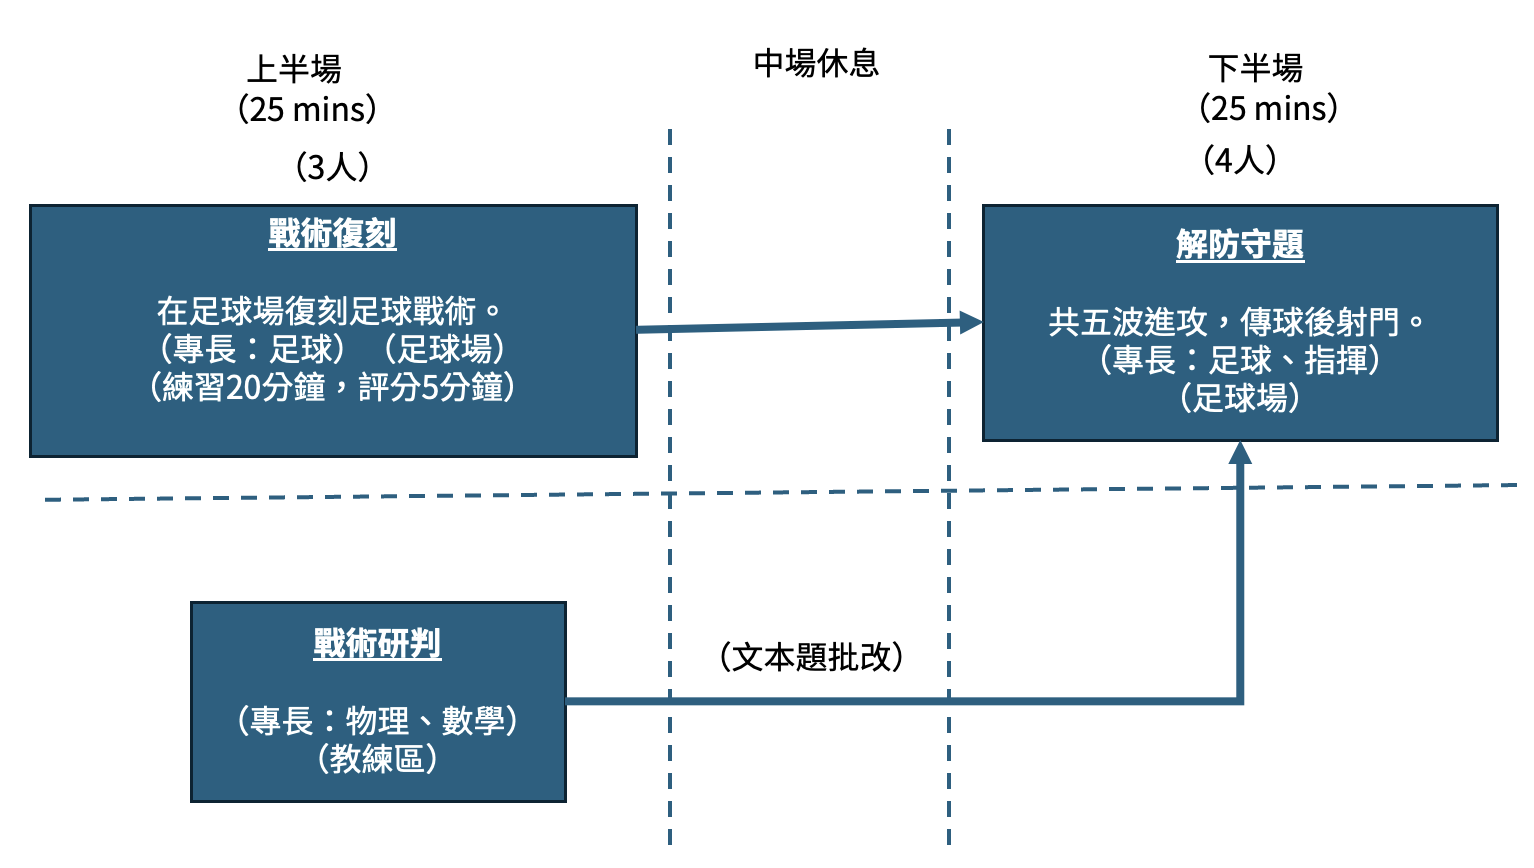
\includegraphics[width=0.92\textwidth]{1.png}

\vspace{0.5em}
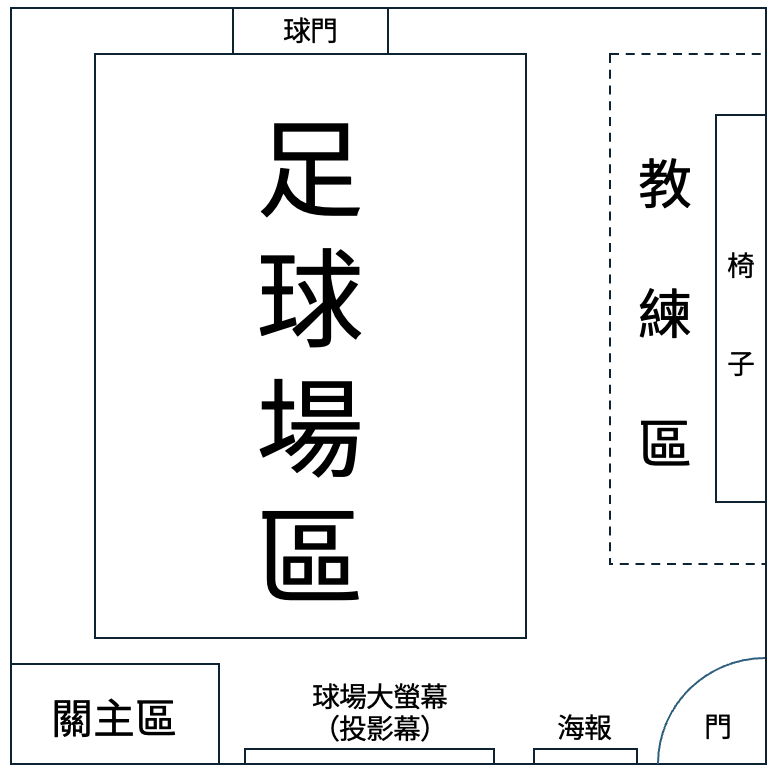
\includegraphics[width=0.92\textwidth]{2.png}
\end{center}

\section*{闖關規則}
\begin{enumerate}
  \item 本關卡共60分鐘，時間分配如關卡流程所示。
  \item 前五分鐘可以打王牌或魔法牌。
  \item 建議分工：戰術復刻約2-3人，物理PDF約2-3人。
  \item 破壞場佈則整關0分。
\end{enumerate}

\section*{上半場}
\subsection*{戰術復刻（270分）}
戰術復刻流程分為兩個步驟，分別為畫跑位及跑戰術。共6個戰術，一個戰術45分。場上會有靜止的防守球員，會站在特定位置，每個防守球員都是3格高的紙箱。

\subsubsection*{畫跑位}
場地會有戰術描述，需請小隊員去找這些戰術描述並依照\textbf{跑位定義}在戰術板（位於戰術區）上畫出\textbf{每次接球}時人及球的位置。畫跑位一題15分。

畫跑位相關規定請見戰術區「戰術復刻評分說明」。

\subsubsection*{跑戰術}
球員要在每個戰術的指定時間內完成戰術語言中的戰術。以每次不同球員的第一次觸球作為\textbf{每次接球}時間，並記錄每拍接球位置。跑戰術一題30分，詳細規定請見「戰術復刻評分說明」。

\subsection*{戰術研判（180分）}
教練區有放置一些戰術資料，裡面有文本題，考點涵蓋物理與數學。其中一組與相對論有關，將作為下半場引入相對論概念的鋪陳。評分規則如下：
\begin{enumerate}
  \item 所有文本題的答案請書寫於答案卷上
  \item 請將所有欲批改的答案卷於上半場結束前交給關主，否則不予計分。分數可以兌換道具，詳情請見教練區之 \texttt{points\_table.pdf}。
\end{enumerate}

\section*{下半場}
\subsection*{解防守題（450分）}
本輪為回合制遊戲，一共五題，一題90分，每題有8回合可以嘗試。教練需依照場上形勢選擇自身想打的戰術，並規劃你們的移動來解決問題。足球場區上有數名防守球員，每個防守球員會有不同的性質，包括瘋狗逼搶員、區域大閘、影子盯人者、路線攔截者及守門員。

而每回合分為進攻回合及防守回合，進攻回合步驟如下：
\begin{enumerate}
  \item \textbf{射門階段}
  \begin{itemize}
    \item 只要選擇\textbf{射門}，回合即結束。
  \end{itemize}
  \item \textbf{移動階段}
  \begin{itemize}
    \item 此階段中每位球員可移動一次。
  \end{itemize}
  \item \textbf{傳球階段}
  \begin{itemize}
    \item 可以傳球一次。
  \end{itemize}
  \item \textbf{結束回合}
  \begin{itemize}
    \item 進攻回合結束後，防守方會進行移動
  \end{itemize}
\end{enumerate}

若能在越短的回合內得分及能符合相對論規則，則分數越高。

在回合結束後大螢幕會秀出防守者的更新位置，請小隊員依照上述位置排防守球員。小隊需依指示將防守者放在格子上後才能進行下一回合。詳細規則請見「防守題評分方式」。

\subsubsection*{黃牌}
下列情形會得到黃牌一張：
\begin{itemize}
  \item 使球出界
  \item 使防守者倒地
  \item 未依規定移動球員
\end{itemize}
得到黃牌後，該回合會重新進行。

\subsubsection*{紅牌}
下列情形會得到紅牌一張：
\begin{itemize}
  \item 以手或手臂碰觸球
  \item 一波進攻中累計兩張黃牌
\end{itemize}
得到紅牌後，該波進攻終止並以零分計算。

\section*{計分方式}
\subsection*{上半場}
每次戰術描述中畫跑位15分，跑戰術30分，6次戰術描述共270分。文本題一共180分。

\subsection*{下半場}
每回合得分計算為
\[
90 \left(1-\frac{\max(0,\ \text{回合數}-4)}{10}\right)\cdot\text{越位係數}\cdot\text{因果律係數}
\]
越位係數為：
\begin{itemize}
  \item 所有觀察者不越位 = 1
  \item 靜止觀察者不越位 = 0.6
  \item 越位 = 0.2
\end{itemize}

因果律係數為：
\begin{itemize}
  \item 所有傳球皆符合因果律 = 1
  \item 有至少一次傳球違反因果律 = 0.5
\end{itemize}

共5題滿分450分。場復100分。

\end{document}
